\documentclass[10pt,a4paper]{article}
\usepackage[a4paper, top=2cm, bottom=1.5cm, left=1.5cm, right=1.5cm]{geometry} % Задать размеры полей.
\usepackage[warn]{mathtext} % Русские символы в формулах. Нужно писать до пакета babel. Указывает, что в формулах используются символы кириллицы, которые по умолчанию печатаются прямым шрифтом.
\usepackage[T2A]{fontenc}
\usepackage[utf8]{inputenc}
\usepackage[russian]{babel}
\usepackage{amsmath}
\usepackage{amssymb}
\usepackage{graphicx}
%\usepackage{floatrow}
\usepackage{booktabs}
\usepackage{wrapfig}
\usepackage{fancyhdr}
\usepackage{multicol}
\usepackage{xcolor}

\usepackage{float}
\usepackage{multirow}

\usepackage{subfigure}

% Объявляем новую команду для переноса строки внутри ячейки таблицы
\newcommand{\specialcell}[2][c]{%
	\begin{tabular}[#1]{@{}c@{}}#2\end{tabular}}

\newcommand{\figref}[1]{(См. рис. \ref{#1})}
\newcommand{\secref}[1]{(См. раздел. \ref{#1})}

\newcommand{\angstrom}{\text{\normalfont\AA}}
\newcommand{\e}[1]{\text{$\cdot10^{#1}$}}
\newcommand{\m}{\; м}
\newcommand{\mm}{\; мм}
\newcommand{\um}{\; мкм}
\newcommand{\A}{\; А}
\newcommand{\V}{\; В}
\newcommand{\uV}{\; мкВ}
\newcommand{\cels}{\; ^\circ С}

\pagestyle{fancy}
\fancyhead{}
\fancyhead[L]{\small Дедков Д.А., Маслов А.С., Измерение энергии первого уровня атома гелия методом электронного возбуждения. МФТИ, 2023 г.}
\fancyhead[R]{}
\fancyfoot[C]{\thepage}

\renewcommand{\cot}{\text{ctg}}

\author{\normalsize Маслов Артём, Дедков Денис \\
	\normalsize группа Б01-108а \\
	\normalsize 16.10.2023}
\date{}

\title{
	\Large Измерение энергии первого уровня атома гелия методом электронного возбуждения \\ 
}

\begin{document}
\maketitle
	
	\subsection*{Цель и задачи работы:}
	\begin{enumerate}
		\item Методом электронного возбуждения измерить энергию первого уровня атома гелия динамическим и статическим методами.
	\end{enumerate}
	
	\subsection*{Описание экспериментальной установки}
	
	Схема экспериментальной установки приведена на рисунке \ref{img:exp_scheme}:
	\begin{figure}[H]
		\centering
		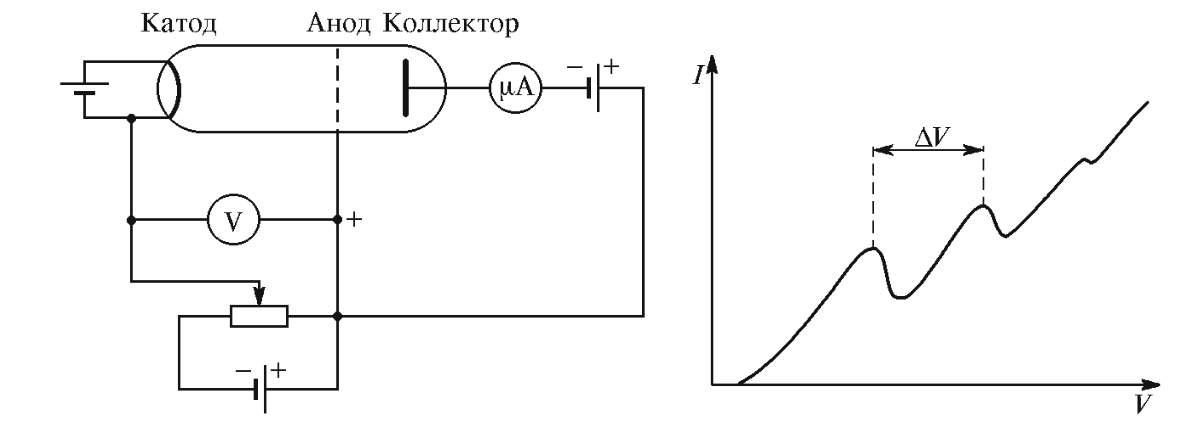
\includegraphics[width=0.8\textwidth]{res/exp_scheme.png}
		\caption{Слева схема экспериментальной установки. Справа схематичный график зависимости тока коллектора от напряжения на аноде.}
		\label{img:exp_scheme}
	\end{figure}

	Разреженный гелий заполняет трехэлектродную лампу. Электроны, испускаемые разогретым катодом, ускоряются в постоянном электрическом поле, созданном между катодом и сетчатым анодом лампы. Передвигаясь от катода к аноду электроны сталкиваются с атомами гелия. Если энергия электрона, налетающего на атом, недостаточна для того, чтобы перевести его в возбуждённое состояние, то возможны только упругие соударения, при которых электроны почти не теряют энергии, так как их масса в тысячи раз меньше массы атомов.
	
	По мере увеличения разности потенциалов между анодом и катодом энергия электронов увеличивается и, в конце концов, оказывается достаточной для возбуждения атомов. При таких неупругих столкновениях одному из атомных электронов передаётся кинетическая энергия налетающего электрона и происходит переход атомного электрона на свободный энергетический уровень или ионизация.
	
	Третьим электродом лампы является коллектор. Между ним и анодом поддерживается небольшое постоянное задерживающее напряжение. Ток коллектора, пропорциональный числу электронов, попадающих на него за секунду, измеряется микроамперметром.
	
	При увеличении потенциала анода ток коллектора сначала растет, но когда энергия электронов становится достаточной для возбуждения атомов, ток коллектора резко уменьшается. Электроны при неупругих столкновениях теряют часть энергии и уже не могут преодолеть задерживающий потенциал. При дальнейшем увеличении потенциала анода, коллекторный ток возрастает. Следующее замедление роста тока происходит в момент, когда часть электроном неупруго сталкивается с атомами два раза. Таким образом, на кривой зависимости тока коллектора от напряжения анода имеется ряд максимумов и минимумов, отстоящих друг от друга на равные расстояния $\Delta V$, которое равно энергии первого возбуждённого состояния.
	
	\begin{figure}[H]
		\centering
		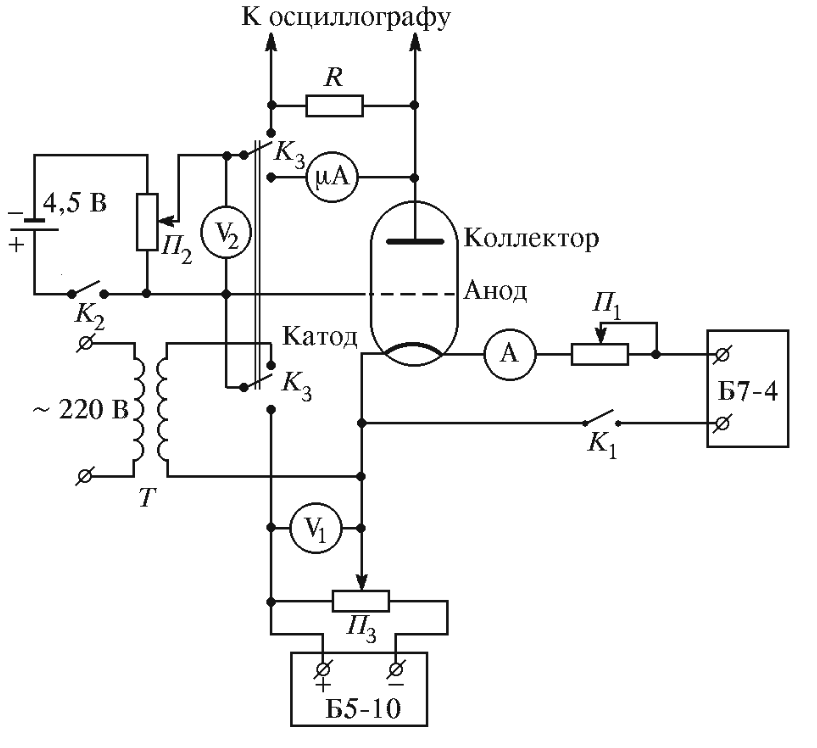
\includegraphics[width=0.8\textwidth]{res/exp_scheme2.png}
		\caption{Слева схема экспериментальной установки. Справа схематичный график зависимости тока коллектора от напряжения на аноде.}
	\end{figure}

	\subsection*{Оборудование и приборы}
	
	Экспериментальная установка $№1.1_4$.
	
	\begin{enumerate}
		\item Трехэлектродная лампа.
		
		\item Вольтметр GDM-8145. Инвентарный номер №51391. Погрешность измерения $\sigma_в = \pm(0.03\%rdg + 4digits)$.
		
		\item Микроамперметр GDM-8145. Инвентарный номер №51399. Погрешность измерения $\sigma_а = \pm (0.3\% rdg + 2 digits)$.
		
		\item Блок питания. Инвентарный номер №410134125745.
	\end{enumerate}
	
	\subsection*{Первичные экспериментальные данные}
		
	В таблицах 1-3 приведены первичные экспериментальные данные статического метода. 
	
	Оценим погрешности первичных экспериментальных данных. Суммарная погрешность измерения тока и напряжения складывается из погрешностей приборов ($\sigma_в = \pm(0.03\%rdg + 4digits)$, $\sigma_а = \pm (0.3\% rdg + 2 digits)$) и случайной погрешностью сигнала, которая определяется шумом в электрической цепи $\sigma_\Sigma = \sqrt{\sigma_{приб.}^2 + \sigma_{случ.}^2}$. Измеряемое значение напряжения флуктуировало примерно на $\pm 0.1 \V$ и не зависело от величины измеряемого напряжения. Поэтому случайную погрешность измерения напряжения оценим величиной этой флуктуации: $\sigma_{н.с.} = \pm 0.01 \V$. При измерении коллекторного тока микроамперметром среднеквадратичное отклонение сигнала от среднего зависело от величины измеряемого тока. Проведя серию измерений среднего значения тока и максимального отклонения измеряемого значения от среднего было установлено, что относительная случайная погрешность измерений составляет примерно $\varepsilon_{т.с.} \approx 2 \%$. Далее считаем, что относительная случайная погрешность измерения тока одинакова во всём диапазоне значений измеряемого сигнала.
	
	\begin{tabular}{cc}
		\begin{tabular}[t]{c}
			Таблица 1. Статический метод. $U_{зад} = 4 \; В$. \\
			\input{gen/tab-dynamic-4.tex}
		\end{tabular}&
		
		\begin{tabular}[t]{c}
			Таблица 2. Статический метод. $U_{зад} = 6 \; В$. \\
			\input{gen/tab-dynamic-6.tex}
		\end{tabular}
	\end{tabular}
	
	\begin{tabular}{c}
		\begin{tabular}[t]{c}
			Таблица 3. Статический метод. $U_{зад} = 8 \; В$. \\
			\input{gen/tab-dynamic-8.tex}
		\end{tabular}
	\end{tabular}

	В таблице 4 приведены первичные экспериментальные данные динамического метода.
	
	\begin{tabular}[t]{c}
		Таблица 4. Динамический метод. \\
		\input{gen/tab-dynamic-xi.tex}
	\end{tabular}
	
	\subsection*{Обработка экспериментальных данных}
		
	\subsubsection*{Динамический метод}
	
	По координатам максимумов и минимумов определим энергию первого возбужденного уровня гелия.
	
	\begin{figure}
		\centering
		\subfigure[]{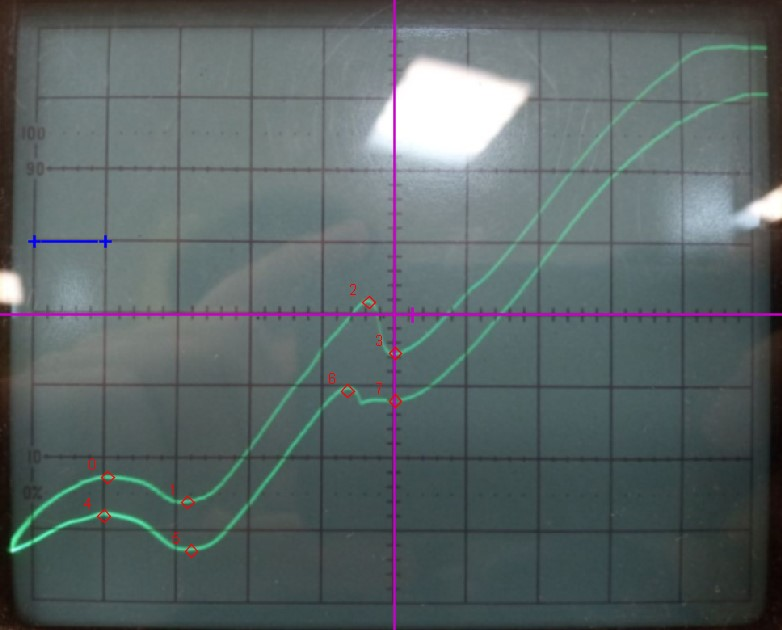
\includegraphics[width=0.3\textwidth]{res/u-4v-p}} 
		\subfigure[]{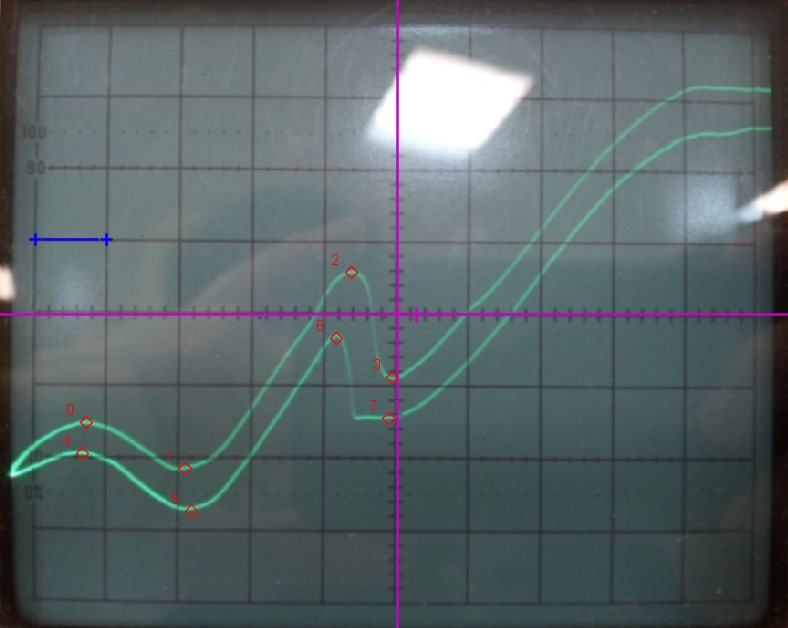
\includegraphics[width=0.3\textwidth]{res/u-6v-p}} 
		\subfigure[]{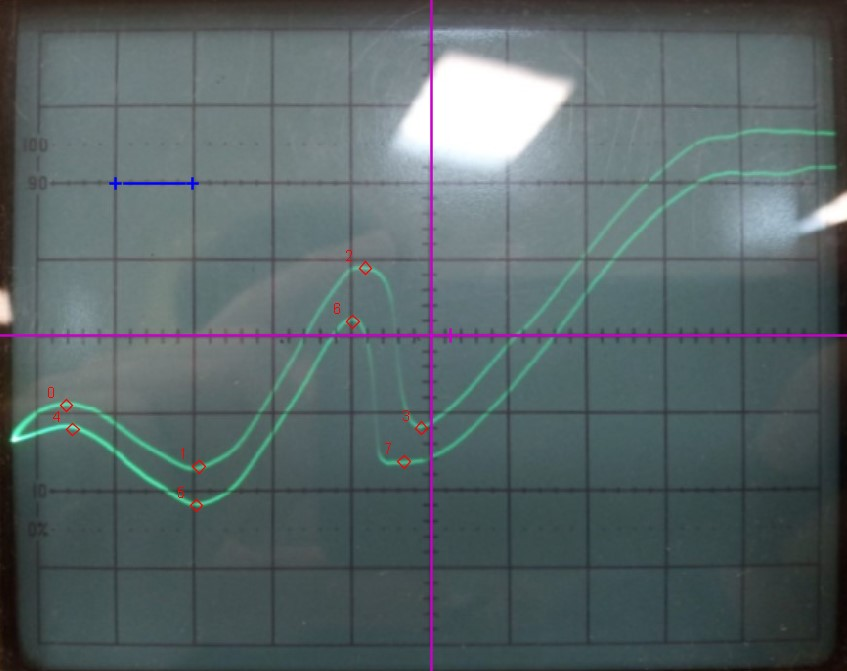
\includegraphics[width=0.3\textwidth]{res/u-8v-p}}  
		\caption{(a) $U = 4\;$В (b) $U = 6\;$В (c) $U = 8\;$В}
		\label{fig:foobar}
	\end{figure}

	\begin{center}
		\begin{tabular}[t]{c}
			Таблица 4. Динамический метод. \\
			\begin{tabular}{cccccccc}
\toprule
$\Delta V_{max}^{(1)}$, В & $\sigma_{\Delta V_{max}^{(1)}}$, В & $\Delta V_{min}^{(1)}$, В & $\sigma_{\Delta V_{min}^{(1)}}$, В & $\Delta V_{max}^{(2)}$, В & $\sigma_{\Delta V_{max}^{(2)}}$, В & $\Delta V_{min}^{(2)}$, В & $\sigma_{\Delta V_{min}^{(2)}}$, В \\
\midrule
18.3 & 0.8 & 14.6 & 0.7 & 17.1 & 0.8 & 14.3 & 0.7 \\
18.6 & 0.8 & 14.5 & 0.7 & 17.7 & 0.8 & 13.8 & 0.7 \\
19.5 & 0.9 & 14.6 & 0.7 & 18.3 & 0.9 & 13.6 & 0.7 \\
\bottomrule
\end{tabular}

		\end{tabular}
	\end{center}


	Погрешность $x_i$ оценим суммой погрешностей отсчета и определения пика. Вторая ошибка варьируется в зависимости от ширины пика. Тогда полная погрешность разности $\sigma_{\Delta V} = \sqrt{\sigma_{x_1}^2 + \sigma_{x_2}^2} $.
	
	Определим среднее значение энергии первого возбужденного уровня гелия $E = 16 \pm 4 \; эВ$. 
	
	\subsubsection*{Статический метод}
	
	Построим график зависимости коллекторного тока от потенциала анода.
	
	\begin{figure}[h]
		\centering
		\includegraphics[width=0.8\textwidth]{gen/fig-vi.pdf}		
	\end{figure}
	
	Определим разности между соседними максимумами и минимумами: \\
	\begin{center}
		\begin{tabular}{|c|c|c|}
			$U_{зад}, \V$ & $\Delta V_{max}, \V$ & $\Delta V_{min}, \V$ \\
			4 & $23.0 \pm 1.4$ & $14.5 \pm 1.4$ \\
			6 & $21.5 \pm 1.4$ & $14.0 \pm 1.4$ \\
			8 & $19.5 \pm 1.4$ & $13.5 \pm 1.4$ \\
		\end{tabular}
	\end{center}

	
	Погрешность измерения $\Delta V$ оценим следующим образом. Точки брались дискретно с шагом $1 \; V$. Сделать шаг меньше в эксперименте не было возможности, так как ручка регулировки напряжения была очень чувствительной. Если на определённом шаге следующее измеренное значение $V_2$ было меньше текущего $V_1$, то это означает о наличии скачка тока на графике $I(V)$. При этом максимум точно находится между $V_1$ и $V_2$. Считаем, что так как не известна информация о математической формуле кривой $I(V)$ и нет возможности провести аппроксимацию (аппроксимация полиномом даст плохой результат, так как на график $I(V)$ не является гладким из-за скачка тока после первого максимума), то пусть вероятность нахождения максимума справа от точки $V_1$ подчиняется гауссовому распределению. Тогда с вероятностью $\approx 98 \%$ максимум находится в интервале $3\sigma = 1 \V$. Тогда погрешность $\sigma(\Delta V) = \sqrt{2} \sigma_V \approx 0.5 \V$.
	
	На графиках видна интересная особенность: резкий спад, приводящий к практически полному совпадению первых максимумов и минимумов. Именно этот скачок приводит к сильному возрастанию ошибки.
	
	Определим среднее значение энергии первого возбужденного состояния атома гелия $E = (18 \pm 4) \; эВ$.
	
	\subsection*{Обсуждение результатов и выводы}
		
	В эксперименте можно наблюдать большую погрешность из-за существенно разных расстояний между соседними минимума и максимумами.
	
	В работе была определена энергия первого возбужденного состояния атома гелия статическим методом $E = (18 \pm 4) \; эВ$.
	
	Была определена энергия первого возбужденного состояния атома гелия динамическим методом  $E = 16 \pm 4 \; эВ$.
	
	Согласно табличным данным энергия, необходимая для перехода атома гелия из основного состояния в первое возбужденное, равна $(19.8 \pm 0.1) \; эВ$.

	
\end{document}